%!TEX root = ../report.tex
\chapter{Introduction}

\textit{P2P is a class of applications that takes advantage of resources -- storage, cycles, content, human presence -- available at the edges of the Internet. Because accessing these decentralized resources means operating in an environment of unstable connectivity and unpredictable IP addresses, P2P nodes must operate outside the DNS system and have significant or total autonomy from central servers.} -- Clay Shirky~\cite{Shirky:2000}


\section{The case for peer-to-peer secure distributed systems}

The recent exposure, by Edward Snowden, of the internet-scale surveillance program performed by the National Security Agency in the United States \cite{} has shown to everybody that anonymity and privacy are inexistent on today's internet. The program was made secretly but sometimes with the complicity of major internet providers and companies, to the detriment of their users.

Notably, last August, Lavabit, an online provider of encrypted email services, decided to terminate its activities to avoid compromising its user data confidentiality \cite{}, soon followed by Silent Circle, a provider of encrypted email, mobile video and voice service provider \cite{}.

On a parallel track, many of the most popular online services, such as Google, Facebook, (Netflix, etc.) have built their business model on profiting from the data user store or generate by interacting with their systems, by selling customized ads or selling the data to third-partys. (Fact-check!) Unfortunately, although no regulation prevents privacy-preserving alternatives from emerging, the enormous profitability of the current business models, combined with the lack of serious large scale funding for developing alternatives, has drawn most of the technical talents to work on improving the existing systems, leaving little viable alternatives for users interested in preserving their privacy.

The need for preserving privacy has been recognized and has lead in the recent years to many projects attempting to develop alternatives to current services. Diaspora, a decentralized privacy-preserving social networking website, has amassed 200,000\$ on the KickStarter crowd funding platform~\footnote{\url{http://www.kickstarter.com/projects/mbs348/diaspora-the-personally-controlled-do-it-all-distr?ref=live}}.

The United Kingdom leading research institutions and companies founded The Horizon Digital Economy Research Institute~\footnote{\url{http://www.horizon.ac.uk/}}, dedicated "to investigate how digital technology may enhance the way we live, work, play and travel in the future". Some of their projects, such as the Internet of Thing, where networking and computing capabilities are aimed at consumer objects and environment, explicitly identify the problematic of defining ownership of data generated with the interaction of the system~\cite{HorizonIoTChallenges:2013}.

Autonomous fully peer-to-peer systems combined with full encryption of all communication and data storage have unique capabilities for preserving the security, privacy and freedom of its users, by connecting its users directly to one another and using resources at the edge of the network. They therefore completely forego any critical centralized component, preventing their appropriation by a malicious or exploitative third-party.

Although peer-to-peer distributed data stores leveraging client-side resources have been built in academia and were hot topics around five years ago, see OceanStore~\cite{} and Farsite~\cite{}, the research community and the industry efforts in distributed systems have now moved to cloud computing, where the infrastructure is owned and operated by single private vendors and rented to users.

One small scottish company, MaidSafe~\footnote{\url{http://maidsafe.net/}}, has been working for over 6 years~\footnote{The earliest recorded version of their website was on december 21st on The Internet Archive \url{http://web.archive.org/web/20071221055035/http://www.maidsafe.net/}} on solving the core issues preventing these technologies from being used in an industrial setting to build alternatives to the services we use online. Their latest release for the core technologies, called Novinet~\footnote{\url{http://www.novinet.com/}}, is now publicly available~\footnote{\url{https://github.com/maidsafe/MaidSafe}} since July 2013 and is licensed both for commercial and open source use. As one of the few active peer-to-peer core technology project, Novinet is really promising.

This report briefly presents the historical developments that have been made on peer-to-peer systems and then use a peer-to-peer internet relay chat application as a case study to evaluate the suitability of MaidSafe libraries for building distributed peer-to-peer online services.


\section{Conceptual Framework}

Peer-to-Peer systems have become mainstream with file sharing technologies, such as Napster (1999) and the Bittorrent (2002) but is still an active area of research, although the research community focus has moved in the last years. This section summarize the content taken from various surveys on different sub-topics ranging from content distribution~\cite{Androutsellis-Theotokis:2004}, network overlays~\cite{Lua:2005}, network management~\cite{Amad:2012}, resource discovery~\cite{Lazaro:2013}, to massively-multiplayer online games~\cite{Yahyavi:2014}.

\subsection{Resource shared}

Computing power,
Bandwidth
Storage

Communication and Collaboration
Distributed Computation
Content Distribution

\subsection{Structure}

Structured
    Topology of the network
    Placement of objects
    Routing and Search functions used to locate objects 
    (implicitly defines a data structure)
    
Unstructured

\subsection{Degree of centralization}

Decentralized, Partially Centralized, Hybrid

\subsection{Non-fonctional requirements}

Security
    Integrity and authenticity
    Privacy and confidentiality
    Availability and persistence
 
Scalability

Performance

Fairness 

Resource Management Capabilities

Semantic Grouping of Information


\subsection{Practical Considerations}

Authentication

Encryption


\section{MaidSafe}

Mission
History
Size
Investors

\subsection{Novinet}

A New Way of looking at Networking by Van Jacobson

Kademlia evolution

\subsection{Current state}




\section{Case Study: peer-to-peer instant messaging system}

\subsection{Operations}
\begin{itemize}
	\item Joining the network
	\item Finding a friend
	\item Sending messages
\end{itemize}

\begin{figure}[htb]
\begin{center}
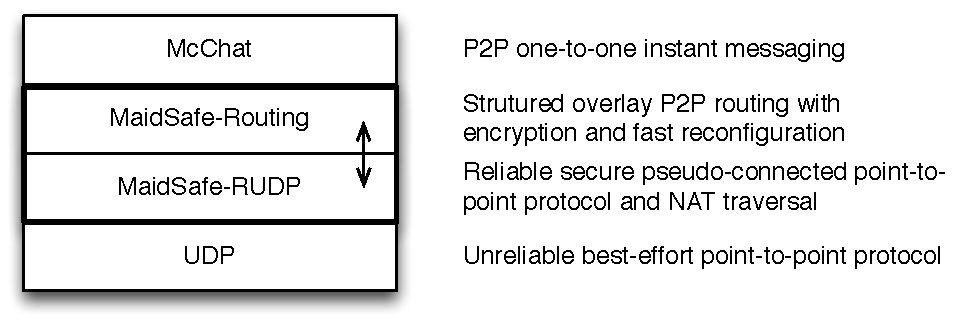
\includegraphics[width=0.8\textwidth]{figures/stack}
\caption{\label{fig:Stack} Stack of technologies}
\end{center}
\end{figure}
